\documentclass[border=4pt]{standalone}
\usepackage[T1]{fontenc}
\usepackage{lmodern}
\usepackage{tikz}
\usetikzlibrary{positioning,arrows.meta}
\begin{document}
\sffamily\footnotesize
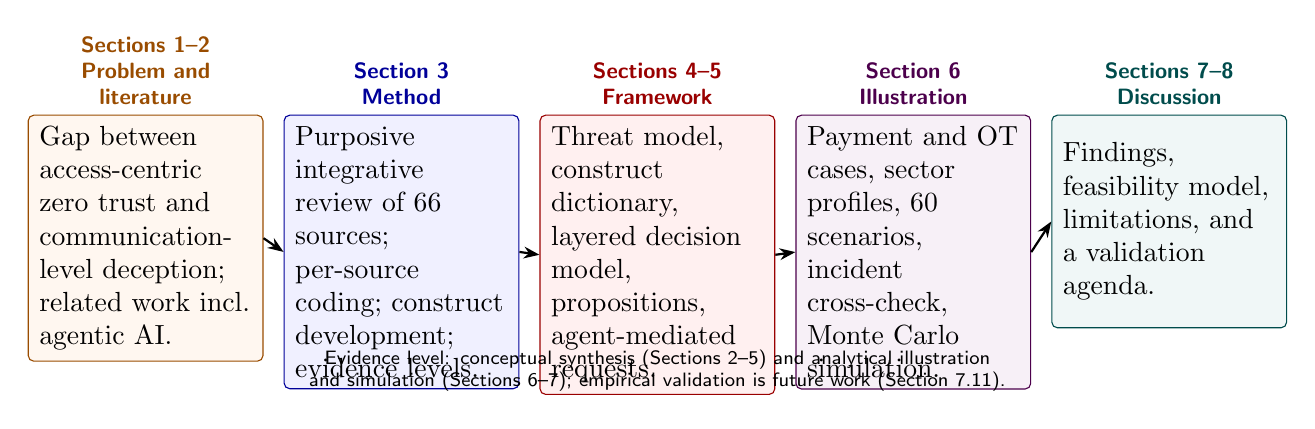
\begin{tikzpicture}[
  st/.style={draw, rounded corners=2pt, align=flush left, text width=27mm, minimum height=27mm, inner sep=4pt, anchor=north},
  hd/.style={font=\sffamily\footnotesize\bfseries, align=center, text width=27mm, anchor=south},
  arr/.style={-{Stealth[length=2mm]}, thick}
]
\foreach \i/\x/\h/\c/\t in {
 1/0/{Sections 1--2\\Problem and literature}/orange/{Gap between access-centric zero trust and communication-level deception; related work incl.\ agentic AI.},
 2/3.25/{Section 3\\Method}/blue/{Purposive integrative review of 66 sources; per-source coding; construct development; evidence levels.},
 3/6.5/{Sections 4--5\\Framework}/red/{Threat model, construct dictionary, layered decision model, propositions, agent-mediated requests.},
 4/9.75/{Section 6\\Illustration}/violet/{Payment and OT cases, sector profiles, 60 scenarios, incident cross-check, Monte Carlo simulation.},
 5/13.0/{Sections 7--8\\Discussion}/teal/{Findings, feasibility model, limitations, and a validation agenda.}}
{
 \node[st, fill=\c!6, draw=\c!60!black] (s\i) at (\x,0) {\t};
 \node[hd, text=\c!60!black] at (s\i.north) {\h};
}
\foreach \a/\b in {1/2,2/3,3/4,4/5} \draw[arr] (s\a.east) -- (s\b.west);
\node[font=\sffamily\scriptsize, align=center, text width=150mm] at (6.5,-3.25)
 {Evidence level: conceptual synthesis (Sections 2--5) and analytical illustration and simulation (Sections 6--7); empirical validation is future work (Section 7.11).};
\end{tikzpicture}
\end{document}
